\section{Design of a Service Mesh Benchmarking Instrument}
\label{sec:system:design}

In this section, we present the design for \textit{Mesh Bench}, a benchmarking instrument for \gls{sm} systems. In \cref{fig:benchmark-design} we depict an overview of the benchmark and all of its components. This design shows how a user interacts with the benchmark, and how it can evaluate the components within the \gls{sut} (see \cref{sec:system:sut}). In the remainder of this section we will introduce the annotated components (as indicated by the black circles \designref{x}) and discuss the functionalities of them.

\begin{figure}[!t]
    \centering
     
    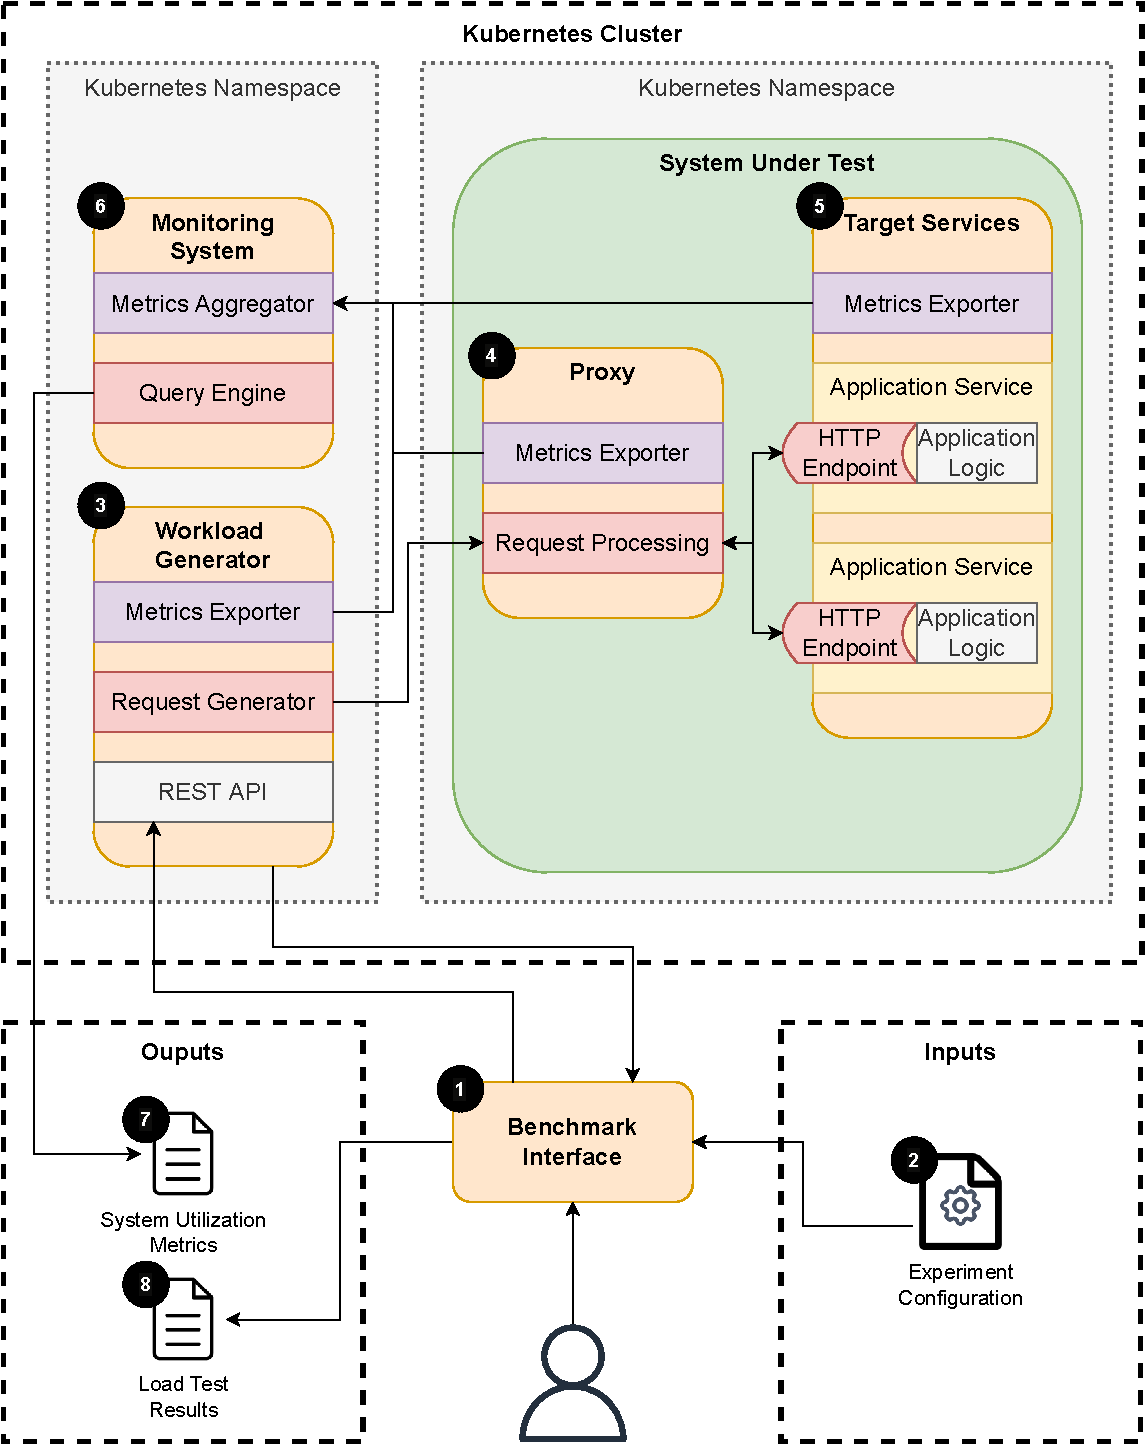
\includegraphics[width=0.9\linewidth]{4_system_design/figures/detailed-benchmark-design.pdf}
    
    \caption[Design of \textit{Mesh Bench}.]{A design overview of \textit{Mesh Bench}, a benchmark for \gls{sm} systems.}
    
    \label{fig:benchmark-design}
\end{figure}



\subsection{Benchmark Interface}
The \textit{Benchmark Interface} \designref{1} is the entry point for the end user and enables them to conduct performance experiments on \gls{sm} systems. The main goal of the Benchmark Interface is to manage experiment executions. The lifecycle of a single experiment consists of three phases. The first phase consists of initialization and configuration. This is done by parsing and processing an \textit{Experiment Configuration} \designref{2}. After this, it instructs the \textit{Workload Generator} \designref{3}, to generate experiment-specific workloads based on the supplied configuration. Once an experiment is finished and the workload generator has reported back to the benchmark interface, it finalizes the experiment and stores the obtained results \designref{8}.

\subsection{Experiment Configuration}
The benchmark consists of several performance experiments, as introduced in \cref{chap:experimental-evaluation}. Each of these experiments consists of several configuration parameters, which allows the user to change several aspects of the experiment. Notable configurations include the ability to modify the type of workload, the frequency of the workload, the duration of the experiment and what type of workload to use, and therefore which target service \designref{5}. These configuration parameters of a single experiment, forms the \textit{Experiment Configuration} \designref{2} and is the primary input of the benchmark interface \designref{1}.


\subsection{Workload Generator}
The \textit{Workload Generator} \designref{3} is used to generate synthetic workloads and measure the performance of the components within the \gls{sut}. This is arguably the most important component in the benchmark, and it has to support various modes of operation to match the functional requirements as defined in \cref{sec:system:requirements-analysis:functional}. The workload generator has to be able to perform load test experiments, in which the \textit{Request Generator} generates a certain application workload for a given \textit{Target Service} \designref{5}. It has to be able to do so in a constant throughput fashion, i.e., a fixed number of requests per second while also supporting a mode that enables us to test the maximum throughput of a given \gls{sut}. Another important aspect is that it should be configurable at run-time, so that the benchmark interface \designref{2} can configure it, allowing us to design various performance related experiments. This aspect is done through the \textit{REST API} as depicted in the benchmark design. The workload generator also exposes system utilization metrics through the \textbf{Metrics Exporter}.

\subsection{Proxy}
The \textit{Proxy} \designref{4} is the core component of a \gls{sm} architecture. The entire benchmark is designed to measure the performance implications of the proxy component. This component varies based on the \gls{sm} system that is evaluated (see \cref{sec:survey:analysis:sm-framework} for the proxies used per \gls{sm} system). Furthermore, it is unmodified, which means that it will intercept all the requests from and to the target service \designref{5}, and do the \textit{Request Processing} as originally intended. However, we do export the resource utilization metrics through the \textit{Metrics Exporter}.

\subsection{Target Services}
At the receiving end of the requests as generated by the workload generator are the \textit{Target Services} \designref{5}. The goal of this component is to mimic a generic service as encountered in a production environment. In this benchmark, we have two \textit{Application Services} to mimic different types of workloads. The first type of service accepts workloads through the \textit{HTTP endpoint}. The second type of service accepts workloads through its \textit{GRPC endpoint}. Both of the backing services accept the synthetic workloads, and perform minimal to no computations on it (\textit{Application Logic)}. This minimizes the impact on end-to-end latencies observed and keeps the resource overheads to a minimum. This allows us to focus on the performance implications of the proxy, instead of the backing services. Just like the other components in the benchmarking system, we export resource utilization metrics through the \textit{Metrics Exporter}.


\subsection{Monitoring System}
The \textit{Monitoring System} \designref{6} is responsible for monitoring the systems within the \textit{Kubernetes Cluster}. This is used primarily to collect resource utilization metrics for all the components within the system through the \textit{Metrics Aggregator}. The monitoring system has to support the collection of these metrics at a fine granularity. More specifically, it has to be able to distinguish resource utilization metrics at a pod and container granularity. This allows us to identify resource utilization patterns for the components of interest. A user should be able to query the aggregated metrics through a \textit{Query Engine} and output these results in a common format to stable storage in a common format \designref{7}.


\subsection{Load Test Results}
The \textit{Load Test Results} \designref{8} are the results created by the \textit{Workload Generator} \designref{3}. These results contain the performance results of an experiment. More specifically, it contains the request latencies as generated by the workload generator. Additionally, it comes with metadata such as the experimental configuration and environment data. 
